\documentclass[conference]{IEEEtran}
\IEEEoverridecommandlockouts
% The preceding line is only needed to identify funding in the first footnote. If that is unneeded, please comment it out.
\usepackage{cite}
\usepackage{url}
\usepackage{hyperref}
\usepackage{amsmath,amssymb,amsfonts}
\usepackage{algorithm}
\usepackage{algpseudocode}
\usepackage{graphicx}
\usepackage{textcomp}
\usepackage{xcolor}
\usepackage{tikz}
\usetikzlibrary{arrows.meta, positioning, calc, fit}
\def\BibTeX{{\rm B\kern-.05em{\sc i\kern-.025em b}\kern-.08em
    T\kern-.1667em\lower.7ex\hbox{E}\kern-.125emX}}
\begin{document}

\title{An LLM-Based Framework for Cross-Market Vehicle Data Normalization\\
\thanks{Identify applicable funding agency here. If none, delete this.}
}

\author{\IEEEauthorblockN{1\textsuperscript{st} Diego Quezada}
\IEEEauthorblockA{\textit{Departamento de Informática} \\
\textit{Universidad Técnica Federico Santa María}\\
Valparaíso, Chile \\
diego.quezadac@sansano.usm.cl}
\and
\IEEEauthorblockN{2\textsuperscript{nd} Carlos Valle}
\IEEEauthorblockA{\textit{Escuela de Ingeniería Informática} \\
\textit{PUCV}\\
Valparaíso, Chile \\
carlos.valle@pucv.cl}
\and
\IEEEauthorblockN{3\textsuperscript{rd} Ricardo Ñanculef}
\IEEEauthorblockA{\textit{Departamento de Informática} \\
\textit{Universidad Técnica Federico Santa María}\\
Valparaíso, Chile \\
jnancu@inf.utfsm.cl}}

\maketitle

\begin{abstract}
The global second-hand vehicle market, valued at approximately USD 1.9 trillion in 2024, is projected to grow at a 9.4\% compound annual growth rate, driven in part by the expansion of online platforms. This expansion has produced a proliferation of heterogeneous vehicle datasets: brand and model names follow no controlled vocabulary, equipment is described in free text across multiple languages, and attribute schemas vary across markets. As a result, most machine learning studies on vehicle data build an ad hoc preprocessing pipeline that does not transfer across sources. We propose a reusable vehicle normalization framework that is agnostic to source schema, language, and market. The framework decomposes normalization into three stages: (i) LLM-based information extraction that maps a raw record to a canonical attribute schema, (ii) dense retrieval of top candidates from a per-attribute knowledge catalog, and (iii) LLM-based entity resolution that either matches the extracted value to a canonical entity or appends it to the catalog as a novel entry. We evaluate each stage in isolation on three public datasets spanning Europe, North America, and North Africa, and conduct ablations over the key design choices at each stage. Finally, we assess the downstream utility of the framework on a used-car resale price prediction task, quantifying the gain from normalized granular attributes over raw inputs. The framework is released as an open-source tool to support reproducible preprocessing of vehicle data across markets.
\end{abstract}

\begin{IEEEkeywords}
LLM, RAG, Information Extraction, Information Retrieval, Entity Resolution

\end{IEEEkeywords}

\section{Introduction}

% Paragraph about the context
The global second-hand car market, valued at approximately USD 1.90 trillion in 2024, is projected to grow at a compound annual growth rate (CAGR) of 9.4\% from 2022 to 2027 \cite{hu2025583}. Key factors driving this growth include rising new vehicle prices, enhanced vehicle financing options, and advancements in online platforms \cite{hu2025583, zacharof}, which facilitate access to inventory and information impacting consumer trust, such as online reviews and ratings \cite{zhang2025decoding}.

% Paragraph about the problem
The expansion of online platforms has produced a proliferation of heterogeneous vehicle datasets across automotive markets. Without a shared standard for representing vehicles, descriptions of the same real-world entity diverge along three axes: \textbf{naming inconsistency}, where the same concept appears under different strings (e.g., ``mercedes'', ``mercedes-benz'', ``mercedes benz''); \textbf{granularity inconsistency}, where the same attribute is expressed at different levels of detail (e.g., ``automatic'' vs.\ ``7-speed DCT''); and \textbf{scope inconsistency}, where a single field conflates values that belong to distinct real-world dimensions (e.g., a \textit{fuel type} column containing both ``petrol'' and ``phev''). Left unaddressed, these inconsistencies propagates through downstream machine learning (ML) pipelines, undermining feature extraction, similarity computation, and ultimately model performance.

% Paragraph about standard efforts
Several standardization efforts have attempted to formalize vehicle data representation, yet none has produced a solution applicable to open, cross-market datasets. The Vehicle Identification Number (VIN), standardized under ISO 3779~\cite{iso3779}, has proven effective within closed industry systems and dealership networks, but its decoding tables are proprietary, vary across manufacturers, and VIN data is rarely present in open datasets. The NHTSA vPIC database~\cite{NHTSAvPIC} decodes VINs into approximately 130 attributes but is restricted to US-market vehicles and excludes condition, usage history, and equipment. The ACES/PIES standards~\cite{AutoCareACES} provide structured fitment data for aftermarket parts in North America, not whole-vehicle attributes. The W3C Automotive Ontology and its \texttt{schema.org} extension~\cite{SchemaOrgAuto} define a minimal set of vehicle properties for web markup, but accept free-form text for key fields and omit trim, equipment, and condition entirely. COVESA's Vehicle Signal Specification (VSS)~\cite{COVESAVSS} standardizes in-vehicle telemetry signals rather than vehicle-as-product attributes, and its own gap analysis acknowledges persistent interoperability issues across OEMs~\cite{COVESAVDMReq}. Together, these efforts address narrow, well-scoped problems within specific industry contexts, leaving the challenge of normalizing heterogeneous vehicle listings from open source datasets largely unresolved. This problem has been repeatedly noted in the vehicle price prediction literature~\cite{electronics12143083, vehicles7030094, 10825740}, where studies report that extensive ad-hoc preprocessing is required for each new dataset and call for standardized representation protocols.

% Paragraph about contribution
In this work, we propose a general vehicle normalization framework that leverages recent advances in large language models (LLMs) applied to information extraction (IE), information retrieval (IR), and entity resolution (ER) to map any raw vehicle description to a normalized, domain-consistent representation suitable for downstream machine learning (ML) tasks. Our framework is open-source and extensible, allowing practitioners to define custom output schemas tailored to their specific attribute requirements, and is designed to serve as a shared baseline for future research on ML applications in the vehicle domain.


\section{Related Work}

\subsection{Vehicle Data Preprocessing in ML}

Every ML study on vehicle data confronts the fact that each dataset uses its own representation: different columns, naming conventions, languages, abbreviations, and attribute domains. In practice, each study builds a tailored preprocessing pipeline from scratch, and none of the resulting transformations transfers to a new dataset or market.

Bergmann and Feuerriegel~\cite{bergmann2025125640} provide the most detailed example of this pattern. Working with 92,239 used car sales from a Swiss retailer, they faced approximately 50,000 unique equipment identifiers represented as short German-language text descriptions (e.g., \textit{``Navigationsfunktion `Discover media' fuer Radiosystem `Composition media'\,''}). Their preprocessing pipeline consisted of three steps: first, they manually selected 18 target equipment categories (e.g., navigation system, alloy rims, park assist) based on the search filters of a Swiss online platform, validated by 51 car dealers; second, they mapped the 50,000 textual descriptions onto these 18 categories using a keyword-based search combined with regular expressions; third, they applied one-hot encoding to produce 18 binary predictors. This pipeline improved prediction performance (MAE) by 3.27\%. Crucially, the authors describe their approach as ``tailored'' to their partner company's data and market. The keyword rules are language-specific (German), the 18 categories reflect Swiss consumer preferences, and the mapping logic would need to be rebuilt for any new market, language, or equipment taxonomy.

Fayyaz et al.~\cite{vehicles7030094} expose how raw vehicle listings resist direct ML application. Working with real-world listing data, they found that transmission entries varied widely (e.g., ``6-Speed A/T'', ``8-Speed PDK'', ``CVT-F''), mileage was stored as strings (e.g., ``10,000 mi.''), and engine specifications were embedded in free text (e.g., ``2.0L 255HP'') requiring regex extraction. They also standardized color names from manufacturer branding (e.g., ``Midnight Black'' mapped to ``Black''). After systematic feature engineering, Linear Regression $R^2$ improved from 0.03 to 0.80, yet the authors acknowledge that their pipeline is dataset-specific. Dutulescu et al.~\cite{electronics12143083} confirm that this problem extends across markets: training deep learning models on a German dataset (300,000+ entries) and evaluating on a Romanian dataset (15,000+ entries), they found that car model embeddings failed for infrequent models and explicitly called for ``a method for dataset standardization across different car markets.'' Madhusudhanan et al.~\cite{10825740} faced similar challenges at larger scale, handling 56 categorical features (make, model, trim, equipment, market region) across approximately 2 million records, where state-of-the-art tabular models could not even process the dataset due to the high cardinality of unstandardized vehicle attributes.

These studies collectively demonstrate that vehicle data preprocessing remains ad-hoc, non-transferable, and a significant engineering bottleneck. Our framework addresses this gap by providing a reusable normalization pipeline that is agnostic to source schema, language, and market.

\subsection{Information Extraction}

IE from product descriptions has evolved from task-specific sequence taggers to general-purpose LLM-based extractors. OpenTag~\cite{zheng2018opentag} formalized product attribute value extraction (AVE) as sequence tagging with a BiLSTM-CRF architecture, achieving 83\% F1 with only 150 annotated samples. Wang et al.~\cite{wang2020aveqa} reformulated AVE as question answering, where each attribute becomes a query and the model identifies answer spans using a shared BERT encoder.

The most relevant line of work for our framework comes from Brinkmann et al. In an initial study~\cite{brinkmann2023chatgpt_ie}, they showed that ChatGPT achieves performance comparable to fine-tuned pre-trained language models (PLMs) for product information extraction while requiring far less training data: a single few-shot example boosted open extraction F1 by approximately 33\%. Their follow-up, ExtractGPT~\cite{brinkmann2024extractgpt}, evaluated GPT-3.5, GPT-4, and Llama-3-70B on attribute-value extraction from unstructured product descriptions, with GPT-4 reaching 85\% F1 and outperforming BERT-based baselines. Most directly relevant to our work, Brinkmann et al.~\cite{brinkmann2024adbis} extended AVE to include \textit{normalization}, exploring GPT-3.5 and GPT-4 for both extracting and normalizing attribute values to a unified scale. On the WDC-PAVE benchmark, GPT-4 achieved 91\% F1 with 10 demonstrations, and the authors found LLMs to be especially strong at name expansion and string wrangling for normalization, which is precisely the capability our framework exploits for vehicle attribute extraction.

Beyond product-specific work, GoLLIE~\cite{sainz2024gollie} demonstrated that encoding annotation guidelines as Python class definitions with docstrings enables high-quality zero-shot IE, outperforming GPT-3.5 on NER tasks. This finding is directly relevant to our approach, where the vehicle attribute schema serves an analogous role as a structured extraction guide.

\subsection{Information Retrieval}

The RAG paradigm, introduced by Lewis et al.~\cite{lewis2020rag}, combines parametric (model weights) and non-parametric (retrieved documents) knowledge by coupling a seq2seq model with a dense vector index. For the retrieval component specifically, Karpukhin et al.~\cite{karpukhin2020dpr} established that learned dual-encoder embeddings (Dense Passage Retrieval) outperform BM25 by 9--19\% absolute in top-20 retrieval accuracy. Izacard et al.~\cite{izacard2022contriever} showed that fully unsupervised dense retrieval via contrastive learning matches BM25 without requiring labeled query-passage pairs, which is particularly relevant when labeled vehicle matching data is scarce.

For efficient nearest-neighbor search over embedding spaces, the FAISS library~\cite{johnson2021faiss, douze2024faiss} provides GPU-optimized algorithms supporting brute-force, inverted file (IVF), product quantization (PQ), and hierarchical navigable small world (HNSW) indexing. On the embedding side, Sentence-BERT~\cite{reimers2019sbert} established the paradigm of pre-computed sentence embeddings for efficient similarity search, while recent models such as E5~\cite{wang2022e5} and BGE~\cite{xiao2024bge} have achieved state-of-the-art results on retrieval benchmarks. Our framework uses HNSW indexes built over sentence embeddings to retrieve candidate values for open-domain vehicle attributes.

\subsection{Entity Resolution}

ER determines whether two surface forms refer to the same real-world entity (e.g., whether ``mercedes'' and ``mercedes-benz'' denote the same brand). Pre-LLM approaches relied on fine-tuning PLMs: Ditto~\cite{li2020ditto} fine-tuned BERT and RoBERTa for entity matching with domain knowledge injection and data augmentation, achieving up to 29\% F1 improvement over prior methods. Narayan et al.~\cite{narayan2022foundation} were the first to cast entity matching as a prompting task for GPT-3, showing that foundation models achieve competitive performance without task-specific fine-tuning.

The most systematic investigation of LLM-based ER comes from the Mannheim group. Peeters and Bizer~\cite{peeters2023chatgpt_em} conducted the first evaluation of ChatGPT for entity matching, finding that it achieves 82.35\% F1 in zero-shot on the WDC Products benchmark, competitive with RoBERTa fine-tuned on 2,000 labeled examples. They explored prompt engineering strategies including similarity-based demonstration selection and matching rule provision. In their comprehensive follow-up, MatchGPT~\cite{peeters2025matchgpt}, they evaluated GPT-4, GPT-4o, and Llama across product and bibliographic datasets. GPT-4 in zero-shot outperformed fine-tuned PLMs by 40--68\% F1 for previously unseen entities, a setting directly analogous to vehicle normalization where new brands, models, and trims continuously appear. They further investigated prompt design, demonstration selection, and matching rule generation, providing a methodological foundation for LLM-based matching in specialized domains. Steiner et al.~\cite{steiner2024finetune_em} complemented this work by exploring fine-tuning LLMs for entity matching, finding that it improves smaller models but can hurt cross-domain transfer for larger ones.

On the efficiency front, Zhang et al.~\cite{zhang2024anymatch} showed that a fine-tuned GPT-2 model achieves quality within 4.4\% F1 of MatchGPT while requiring four orders of magnitude fewer parameters, demonstrating that cost-effective deployment is feasible. Wang et al.~\cite{wang2025comem} compared three LLM matching strategies (binary matching, comparing, and selecting from candidates) and found the selecting strategy most cost-effective.


\section{Method}
\label{sec:method}

We frame vehicle normalization as a three-stage pipeline
(Fig.~\ref{fig:pipeline}). A raw record $\mathbf{x}$ is first serialized
and passed to an LLM that jointly extracts candidate attribute values
$\hat{\mathbf{x}} = (\hat{a}_1, \dots, \hat{a}_m)$ (\textit{information
extraction}). Closed-domain attributes are emitted directly; each
open-domain attribute $\hat{a}_j$ is then encoded and matched against a
knowledge catalog $\mathcal{K}_j$ to retrieve its top-$k$ canonical
candidates $\mathcal{R}_j$ (\textit{retrieval}). Finally, an LLM resolver
decides whether any candidate $c_i \in \mathcal{R}_j$ refers to the same
real-world entity as $\hat{a}_j$; if one does, it replaces $\hat{a}_j$,
otherwise $\hat{a}_j$ is kept as a novel entity and appended to
$\mathcal{K}_j$ (\textit{entity resolution}). The remainder of this
section formalizes each stage.

\begin{figure}[t]
\centering
\resizebox{\columnwidth}{!}{%
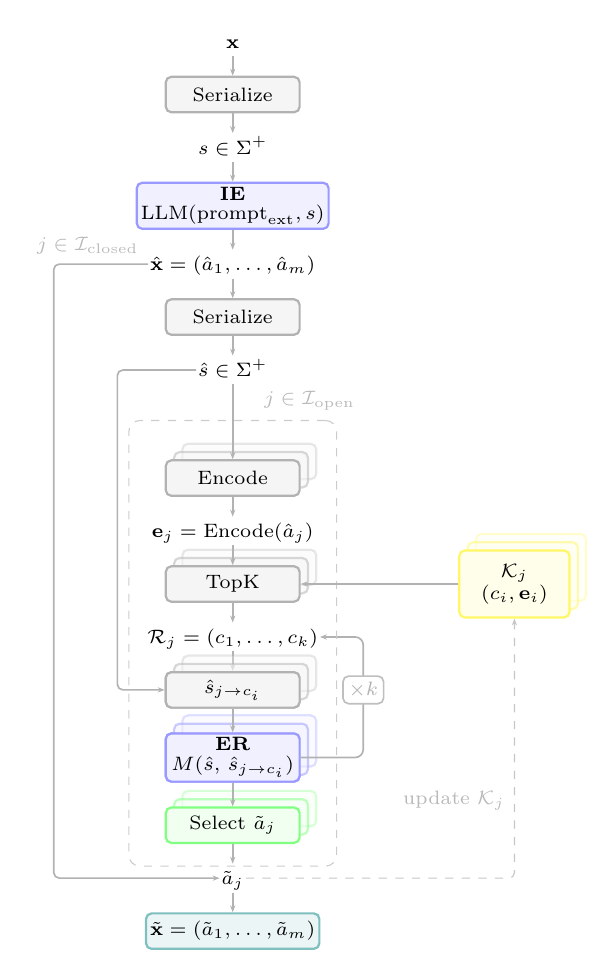
\begin{tikzpicture}[
    node distance=0.18cm and 0.3cm,
    every node/.style={font=\scriptsize},
    op/.style={draw, rounded corners=2pt, fill=gray!8, 
               draw=gray!60, thick, minimum height=0.45cm,
               minimum width=1.7cm, inner sep=1.5pt, align=center},
    llm/.style={draw, rounded corners=2pt, fill=blue!6, 
                draw=blue!40, thick, minimum height=0.45cm,
                minimum width=1.7cm, inner sep=1.5pt, align=center},
    sel/.style={draw, rounded corners=2pt, fill=green!6,
                draw=green!50, thick, minimum height=0.45cm,
                minimum width=1.7cm, inner sep=1.5pt, align=center},
    ops/.style={draw, rounded corners=2pt, fill=gray!8, 
                draw=gray!60, thick, minimum height=0.45cm,
                minimum width=1.7cm, inner sep=1.5pt},
    llms/.style={draw, rounded corners=2pt, fill=blue!6, 
                 draw=blue!40, thick, minimum height=0.65cm,
                 minimum width=1.7cm, inner sep=1.5pt},
    sels/.style={draw, rounded corners=2pt, fill=green!6,
                 draw=green!50, thick, minimum height=0.45cm,
                 minimum width=1.7cm, inner sep=1.5pt},
    cats/.style={draw, rounded corners=2pt, fill=yellow!8, 
                 draw=yellow!60, thick, minimum width=1.4cm,
                 minimum height=0.85cm, inner sep=1.5pt},
    dat/.style={align=center, inner sep=0.5pt, 
                text height=1.6ex, text depth=0.5ex},
    cat/.style={draw, rounded corners=2pt, fill=yellow!8, 
                draw=yellow!60, thick, minimum width=1.4cm,
                minimum height=0.85cm, inner sep=1.5pt, align=center},
    outnode/.style={draw, rounded corners=2pt, fill=teal!8,
                    draw=teal!50, thick, minimum height=0.45cm,
                    minimum width=1.7cm, inner sep=1.5pt, align=center},
    dm/.style={font=\scriptsize\itshape, text=gray!55},
    arr/.style={-{Stealth[length=2.5pt]}, semithick, gray!60},
    darr/.style={-{Stealth[length=2.5pt]}, gray!45, dashed},
    lb/.style={font=\scriptsize, text=gray!55},
    loopbox/.style={draw=gray!40, dashed, rounded corners=4pt, inner sep=5pt},
    soff/.style={xshift=3pt, yshift=3pt},
    soff2/.style={xshift=6pt, yshift=6pt},
]

% Standard gaps:
%   text label between arrows: 0.25cm above and below
%   block to block (no text):  0.3cm
%   block to stacked block:    same 0.3cm (shadows use same position)

% ===== TOP: shared pipeline =====
\node[dat] (x) {$\mathbf{x}$};

\node[op, below=0.25cm of x] (ser) {Serialize};
\draw[arr] (x) -- (ser);

\node[dat, below=0.25cm of ser] (s) {$s \in \Sigma^+$};
\draw[arr] (ser) -- (s);

\node[llm, below=0.25cm of s] (ie) 
    {\textbf{IE}\\[-1pt] $\mathrm{LLM}(\mathrm{prompt}_{\mathrm{ext}}, s)$};
\draw[arr] (s) -- (ie);

\node[dat, below=0.25cm of ie] (xhat) 
    {$\hat{\mathbf{x}} = (\hat{a}_1, \dots, \hat{a}_m)$};
\draw[arr] (ie) -- (xhat);

\node[op, below=0.25cm of xhat] (ser2) {Serialize};
\draw[arr] (xhat) -- (ser2);

\node[dat, below=0.25cm of ser2] (shat) {$\hat{s} \in \Sigma^+$};
\draw[arr] (ser2) -- (shat);

% ===== OUTER STACKED SECTION =====

% Encode (extra gap below shat for dashed box label)
\node[ops, soff2, below=0.95cm of shat, opacity=0.3] (enc_s2) {};
\node[ops, soff,  below=0.95cm of shat, opacity=0.5] (enc_s1) {};
\node[op,         below=0.95cm of shat]              (enc)    {Encode};
\draw[arr] (shat) -- (enc);

\node[dat, below=0.25cm of enc] (ej) 
    {$\mathbf{e}_j = \mathrm{Encode}(\hat{a}_j)$};
\draw[arr] (enc) -- (ej);

% TopK
\node[ops, soff2, below=0.25cm of ej, opacity=0.3] (topk_s2) {};
\node[ops, soff,  below=0.25cm of ej, opacity=0.5] (topk_s1) {};
\node[op,         below=0.25cm of ej]              (topk)    {TopK};
\draw[arr] (ej) -- (topk);

% Rj text splitting the arrow
\node[dat, below=0.25cm of topk] (rj) 
    {$\mathcal{R}_j = (c_1, \dots, c_k)$};
\draw[arr] (topk) -- (rj);

% ===== INNER SECTION =====

\node[op,  below=0.25cm of rj] (sub) {$\hat{s}_{j \to c_i}$};
\draw[arr] (rj) -- (sub);

\node[llm, below=0.3cm of sub] (er) 
    {\textbf{ER}\\[-1pt] $M(\hat{s},\, \hat{s}_{j \to c_i})$};

% Shadow blocks
\node[ops,  soff2, opacity=0.3] at (sub) {};
\node[ops,  soff,  opacity=0.5] at (sub) {};
\node[llms, soff2, opacity=0.3] at (er) {};
\node[llms, soff,  opacity=0.5] at (er) {};

% Redraw front blocks on top
\node[op]  at (sub) {$\hat{s}_{j \to c_i}$};
\node[llm] at (er) {\textbf{ER}\\[-1pt] $M(\hat{s},\, \hat{s}_{j \to c_i})$};
\draw[arr] (sub) -- (er);

% Arrow from shat to sub block directly
\draw[arr, rounded corners=2pt] 
    (shat.west) -- ++(-1.0,0) |- (sub.west);

% ×k loop arrow
\draw[arr, rounded corners=3pt]
    (er.east) -| 
    ([xshift=0.55cm]rj.east) --
    (rj.east);

% ×k badge
\node[draw=gray!50, fill=white, semithick, rounded corners=2pt,
      font=\scriptsize\bfseries, text=gray!60, inner sep=2pt,
      minimum width=0.5cm, minimum height=0.35cm]
    at ([xshift=0.55cm]rj.east |- sub) {$\times k$};

% ===== SELECT (outer stacked) =====
\node[sels, soff2, below=0.3cm of er, opacity=0.3] (sel_s2) {};
\node[sels, soff,  below=0.3cm of er, opacity=0.5] (sel_s1) {};
\node[sel,         below=0.3cm of er]              (select) 
    {Select $\tilde{a}_j$};
\draw[arr] (er) -- (select);

% ===== Output =====
% Combined label as a text-between-arrows node — vertically centered on the arrow
\node[dat, below=0.25cm of select] (aj)
    {$\tilde{a}_j$}; %
\draw[arr] (select) -- (aj);

\node[outnode, below=0.25cm of aj] (output) 
    {$\tilde{\mathbf{x}} = (\tilde{a}_1, \dots, \tilde{a}_m)$};
\draw[arr] (aj) -- (output);

% ===== Outer loop box (aj is OUTSIDE) =====
\node[loopbox, 
      fit=(enc)(enc_s2)(ej)(rj)(sub)(er)(select)(sel_s2),
      inner xsep=6pt, inner ysep=8pt] (outerloop) {};

\node[lb, anchor=south east] at ([xshift=0.35cm]outerloop.north east)
    {$j \in \mathcal{I}_{\mathrm{open}}$};

% ===== Catalog =====
\node[cats, soff2, right=2.0cm of topk, opacity=0.3] (cat_s2) {};
\node[cats, soff,  right=2.0cm of topk, opacity=0.5] (cat_s1) {};
\node[cat,         right=2.0cm of topk]              (catalog) 
    {$\mathcal{K}_j$\\
     $(c_i, \mathbf{e}_i)$};
\draw[arr] (catalog) -- (topk);

\draw[darr, rounded corners=2pt] 
    (aj.east) -| (catalog.south)
    node[lb, left, pos=0.65] 
    {update $\mathcal{K}_j$};

% ===== Closed-domain bypass: solid gray arrow into aj from the left =====
\draw[arr, rounded corners=2pt] 
    (xhat.west) -- ++(-1.2,0) |- (aj.west);
\node[lb, anchor=south east] at ([xshift=-0cm, yshift=0cm]xhat.west)
    {$j \in \mathcal{I}_{\mathrm{closed}}$};

\end{tikzpicture}
}
\caption{Vehicle normalization pipeline. A raw record $\mathbf{x}$ is serialized and fed to an LLM that jointly extracts candidate attribute values $\hat{\mathbf{x}}$ (IE). Closed-domain attributes ($\mathcal{I}_{\text{closed}}$) bypass the loop and are emitted as-is. Each open-domain attribute ($\mathcal{I}_{\text{open}}$, dashed box) is encoded into $\mathbf{e}_j$, its top-$k$ canonical candidates $\mathcal{R}_j$ are retrieved from catalog $\mathcal{K}_j$ via HNSW, and each candidate $c_i$ is substituted into $\hat{s}_{j \to c_i}$ and tested by an LLM entity resolver $M(\cdot,\cdot)$. Stacked blocks represent one instance per open-domain attribute, and the $\times k$ arrow indicates that for each retrieved value we repeat the substitution-and-resolution process within each block. Select returns the first matching $c_{i^*}$; otherwise $\hat{a}_j$ is kept as a novel entity and the catalog is expanded (dashed feedback). See Algorithm~\ref{algo:normalization}.}
\label{fig:pipeline}
\end{figure}


Let the normalized vehicle schema consist of $m$ attributes
$A_1, A_2, \dots, A_m$, where each attribute $A_j$ is associated with a
domain $\mathcal{V}_j$ of valid values. Attribute domains are partitioned
into two types:
\begin{equation}
\mathcal{V}_j =
\begin{cases}
\mathcal{V}_j^{\text{closed}} & \text{if } j \in \mathcal{I}_{\text{closed}}, \\[4pt]
\mathcal{V}_j^{\text{open}} & \text{if } j \in \mathcal{I}_{\text{open}}.
\end{cases}
\end{equation}
A \textit{closed-domain} attribute has a domain that is fully specified
in advance and does not change during normalization. This includes both
finite categorical sets and numerical ranges (e.g., mileage
$\in \mathbb{R}^+$). An \textit{open-domain} attribute (e.g., brand,
model) has a domain that grows as the system encounters previously
unseen entities.


The normalized vehicle space is the Cartesian product of all attribute
domains:
\begin{equation}
\tilde{\mathcal{X}} = \prod_{j=1}^{m} \mathcal{V}_j.
\end{equation}
Vehicle normalization is formulated as a mapping
\begin{equation}
\phi: \Sigma^+ \to \tilde{\mathcal{X}},
\end{equation}
that takes a serialized vehicle representation
$s = \text{Serialize}(\mathbf{x}) \in \Sigma^+$, where $\mathbf{x}$ is
the raw input record and $\Sigma$ denotes the character alphabet, and
produces $\phi(s) = \tilde{\mathbf{x}} \in \tilde{\mathcal{X}}$. For
tabular datasets, $\text{Serialize}$ concatenates column names with their
values (e.g., \textit{col1: val1, col2: val2, \dots}); for free-text
descriptions, the input is used directly.

\paragraph{Knowledge catalog.}
For each open-domain attribute $A_j$ with
$j \in \mathcal{I}_{\text{open}}$, we maintain a knowledge catalog:
\begin{equation}
\mathcal{K}_j = \{(c_1, \mathbf{e}_1), \dots,
(c_{|\mathcal{K}_j|}, \mathbf{e}_{|\mathcal{K}_j|})\},
\end{equation}
where each pair $(c_i, \mathbf{e}_i)$ consists of a canonical entity
value $c_i \in \mathcal{V}_j^{\text{open}}$ and its embedding
$\mathbf{e}_i = \text{Encode}(c_i) \in \mathbb{R}^{d}$. Any text
encoder may serve as the encoding function.


\paragraph{Information extraction.}
Given a serialized vehicle description $s$, a single LLM call extracts
candidate values for all attributes simultaneously:
\begin{equation}
\hat{\mathbf{x}} = (\hat{a}_1, \dots, \hat{a}_m) =
\text{LLM}(\text{prompt}_{\text{ext}}, s).
\end{equation}
For closed-domain attributes, the extracted value is used directly as
$\tilde{a}_j = \hat{a}_j$, since the prompt constrains the LLM output to
$\mathcal{V}_j^{\text{closed}}$. For open-domain attributes, the
candidate $\hat{a}_j$ is passed to the retrieval and resolution steps
described below.

\paragraph{Information retrieval.}
For each open-domain attribute $A_j$, the extracted candidate is embedded
as $\mathbf{e}_j = \text{Encode}(\hat{a}_j)$, and the top-$k$ most
similar canonical entities are retrieved from catalog $\mathcal{K}_j$:
\begin{equation}
\mathcal{R}_j = \operatorname{top\text{-}k}_{(c_i, \mathbf{e}_i)
\in \mathcal{K}_j}\;
\text{sim}(\mathbf{e}_j, \mathbf{e}_i), \quad
\text{sim}(\mathbf{u}, \mathbf{v}) =
\frac{\mathbf{u}^\top \mathbf{v}}
{\|\mathbf{u}\|_2 \, \|\mathbf{v}\|_2}.
\end{equation}
The candidates in $\mathcal{R}_j$ are ranked in decreasing order of
similarity.

\paragraph{Entity resolution.}
Given the extracted attributes $\hat{\mathbf{x}}$ and the ranked
candidates $\mathcal{R}_j = (c_1, c_2, \dots, c_k)$ for each
open-domain attribute $A_j$, we compare two serialized vehicle
descriptions. Let
\begin{equation}
\hat{s} = \text{Serialize}(\hat{\mathbf{x}})
\end{equation}
be the serialization of the extracted attributes. For each candidate
$c_i \in \mathcal{R}_j$, we construct a variant in which the value of
attribute $A_j$ is replaced by $c_i$:
\begin{equation}
\hat{s}_{j \to c_i} = \text{Serialize}(\hat{a}_1, \dots, c_i, \dots, \hat{a}_m).
\end{equation}
The LLM then evaluates whether both descriptions refer to the same
vehicle:
\begin{equation}
M(\hat{s},\, \hat{s}_{j \to c_i}) =
\text{LLM}(\text{prompt}_{\text{res}},\, \hat{s},\,
\hat{s}_{j \to c_i}) \in \{0, 1\}.
\end{equation}
All $k$ candidates are evaluated and the normalized value is:
\begin{equation}
\tilde{a}_j =
\begin{cases}
c_{i^*}, & i^* = \min\{i : m_i = 1\}, \\[4pt]
\hat{a}_j & \text{otherwise (novel entity),}
\end{cases}
\end{equation}
where $m_i = M(\hat{s},\, \hat{s}_{j \to c_i})$.
In the novel-entity case, the catalog is expanded:
$\mathcal{K}_j \leftarrow \mathcal{K}_j \cup
\{(\hat{a}_j, \text{Encode}(\hat{a}_j))\}$.

Algorithm~\ref{algo:normalization} summarizes the complete pipeline.

\begin{algorithm}
\caption{Vehicle Normalization.}
\label{algo:normalization}
\begin{algorithmic}[1]
\Require Raw vehicle record $\mathbf{x}$,
Catalogs $\{\mathcal{K}_j\}_{j \in \mathcal{I}_{\text{open}}}$
\Ensure Normalized representation
$\tilde{\mathbf{x}} = (\tilde{a}_1, \dots, \tilde{a}_m)$

\State $s \gets \text{Serialize}(\mathbf{x})$
\State $\hat{\mathbf{x}} \gets
\text{LLM}(\text{prompt}_{\text{ext}}, s)$

\For{$j \in \mathcal{I}_{\text{closed}}$}
    \State $\tilde{a}_j \gets \hat{a}_j$
\EndFor

\State $\hat{s} \gets \text{Serialize}(\hat{\mathbf{x}})$
\For{$j \in \mathcal{I}_{\text{open}}$}
    \State $\mathbf{e}_j \gets \text{Encode}(\hat{a}_j)$
    \State $\mathcal{R}_j \gets
    \operatorname{TopK}_{(c_i, \mathbf{e}_i) \in \mathcal{K}_j}
    \text{sim}(\mathbf{e}_j, \mathbf{e}_i)$
    \For{$c_i \in \mathcal{R}_j$ in ranked order}
        \State $\hat{s}_{j \to c_i} \gets
        \text{Serialize}(\hat{a}_1, \dots, c_i, \dots, \hat{a}_m)$
        \State $m_i \gets M(\hat{s},\, \hat{s}_{j \to c_i})$
    \EndFor
    \If{$\exists\, i : m_i = 1$}
        \State $i^* \gets \min\{i : m_i = 1\}$
        \State $\tilde{a}_j \gets c_{i^*}$
    \Else
        \State $\tilde{a}_j \gets \hat{a}_j$
        \Comment{novel entity}
        \State $\mathcal{K}_j \leftarrow \mathcal{K}_j \cup
        \{(\hat{a}_j, \text{Encode}(\hat{a}_j))\}$
    \EndIf
\EndFor

\State \Return $\tilde{\mathbf{x}} = (\tilde{a}_1, \dots, \tilde{a}_m)$
\end{algorithmic}
\end{algorithm}

\section{Experiments}

We evaluate each component (IE, IR, ER) in isolation, assembling a dedicated
labeled dataset per task and reporting metrics appropriate to each.

\subsection{Experimental Setup}
\label{sec:setup}

\textbf{Schema.}
Table~\ref{tab:schema} lists the $m = 28$ attributes of the schema used
in this study, and Table~\ref{tab:catalog} specifies the domain
$\mathcal{V}_j^{\text{closed}}$ of each closed-domain categorical
attribute (numerical closed-domain attributes are omitted from the table;
\textit{year} and \textit{doors} take integer values, while the remaining
numerical attributes take positive real values). Of the 28 attributes, four are open-domain
($|\mathcal{I}_{\text{open}}| = 4$): \textit{brand}, \textit{model},
\textit{submodel}, and \textit{trim level}; the remaining 24 are
closed-domain. Numerical attributes with a physical unit are represented
as value/unit pairs (e.g.\ \textit{mileage} paired with \textit{mileage
unit}), where the unit is itself a closed-domain attribute whose domain
covers the conventions found across the target markets. The decomposition
resolves the three inconsistency axes identified in the introduction: the
separation of \textit{energy source}, \textit{propulsion system}, and
\textit{fuel type} addresses scope inconsistency, while the separation of
\textit{transmission type}, \textit{technology}, and \textit{gears}
addresses granularity inconsistency.

\begin{table}[htbp]
\caption{Proposed Normalized Schema ($m = 28$)}
\begin{center}
\footnotesize
\begin{tabular}{|l|l|}
\hline
\textbf{Attribute} & \textbf{Description} \\
\hline
Brand$^\dagger$        & Vehicle manufacturer \\
Model$^\dagger$        & Base vehicle model name \\
Submodel$^\dagger$     & Specific variant of the vehicle model \\
Trim level$^\dagger$   & Feature and styling package \\
Year                   & Model year of the vehicle \\
Mileage                & Numeric odometer reading \\
Mileage unit           & Unit for mileage \\
Body type              & Physical structure and shape \\
Transmission type      & Type of transmission system \\
Transmission tech.     & Specific transmission mechanism \\
Transmission gears     & Number of gear ratios \\
Energy source          & Main energy source powering the vehicle \\
Propulsion system      & Configuration of the propulsion system \\
Fuel type              & Specific fuel used by the vehicle \\
Drive type             & Wheels receiving power from the drivetrain \\
Engine size            & Numeric engine displacement value \\
Engine size unit       & Unit for engine size \\
Engine power           & Numeric maximum power output value \\
Engine power unit      & Unit for engine power \\
Engine aspiration      & Air intake method \\
Injection type         & Fuel injection method \\
Cylinders              & Number of cylinders in the engine \\
Condition              & Vehicle condition as reported by the seller \\
Color                  & Exterior body color \\
Doors                  & Number of doors on the vehicle body \\
Fuel consumption       & Numeric fuel efficiency value \\
Fuel consumption unit  & Unit for fuel consumption \\
Equipment              & Set of standardized features and equipment \\
\hline
\multicolumn{2}{l}{$^\dagger$Open-domain attribute.} \\
\end{tabular}
\label{tab:schema}
\end{center}
\end{table}

\begin{table}[htbp]
\caption{Domain of Closed-Domain Categorical Attributes}
\begin{center}
\footnotesize
\begin{tabular}{|p{2.2cm}|p{5.4cm}|}
\hline
\textbf{Attribute} & \textbf{Domain} \\
\hline
Body type & sedan, hatchback, suv, crossover, coupe, convertible, wagon, pickup, van, minivan, roadster, other \\
\hline
Drive type & fwd, rwd, awd, 4wd, other \\
\hline
Transmission type & manual, automatic, semi-automatic \\
\hline
Transmission tech. & tc, cvt, sct, dct, other \\
\hline
Energy source & fossil, hybrid, electric, other \\
\hline
Propulsion system & icev, ev, pev, bev, hev, mhv, phev, erev, fcev, pfcev, other \\
\hline
Fuel type & petrol, diesel, cng, lpg, lng, methanol, propane, hydrogen, other \\
\hline
Engine aspiration & natural, turbo, supercharger, other \\
\hline
Injection type & direct, indirect, dual, other \\
\hline
Mileage unit & km, mi \\
\hline
Engine size unit & l, cc \\
\hline
Engine power unit & kw, ps, hp \\
\hline
Fuel cons. unit & l/100km, mpg, km/l \\
\hline
Condition & new, excellent, very good, good, fair, poor, salvage \\
\hline
Color & black, white, silver, grey, red, blue, green, yellow, orange, brown, beige, gold, purple, other \\
\hline
\end{tabular}
\label{tab:catalog}
\end{center}
\end{table}

\textbf{Retriever.}
Open-domain attributes are indexed with FAISS HNSW ($M = 32$,
$\mathit{ef}_{\mathrm{search}} = 64$). We set $k = 5$: since each
retrieved candidate triggers one LLM call in the ER stage, $k$ directly
controls cost, and $k = 5$ balances recall headroom against LLM call
budget.

\textbf{Models.}
All extraction and entity resolution LLM calls use OpenAI's
\textit{gpt-4.1-mini}. Candidate embeddings for open-domain attributes
are computed with OpenAI's \textit{text-embedding-3-small} ($d = 1{,}536$).

\subsection{Datasets}

Our experiments draw on three publicly available automotive listing datasets
covering distinct geographic markets, schema conventions, and languages,
summarized in Table~\ref{tab:datasets}. AutoScout24 is a European dataset with
fully structured fields. Craigslist is a North American dataset characterized
by informal free-text descriptions, and its 29{,}667 nominal model values
reflect raw seller input rather than a controlled vocabulary. MuCars~\cite{tabarnoust2024mucars} is a
Moroccan dataset with several market-specific attributes, including Fiscal
Power as a tax-based engine category rather than a direct power measurement.
The heterogeneity across markets and naming conventions makes these three
sources well suited for evaluating the robustness of the normalization method.

\begin{table}[htbp]
\caption{Dataset Statistics}
\begin{center}
\begin{tabular}{|l|r|r|r|r|l|}
\hline
\textbf{Dataset} & \textbf{Listings} & \textbf{Brands} & \textbf{Models} & \textbf{Cols} & \textbf{Region} \\
\hline
AutoScout24 & 251,079 & 47  & 1,312  & 15 & Europe \\
Craigslist  & 426,880 & 42  & 29,667 & 26 & North America \\
MuCars      & 101,896 & 81  & 1,049  & 15 & Morocco \\
\hline
\end{tabular}
\label{tab:datasets}
\end{center}
\end{table}

\subsection{Information Extraction}
\label{sec:eval_ie}

\textbf{Rationale.}
Evaluating the extraction stage requires labeled pairs
$(s, \hat{\mathbf{x}}^*)$ where $\hat{\mathbf{x}}^* = (\hat{a}_1^*, \dots,
\hat{a}_m^*)$ is the correct extraction for description $s$. We use a
three-model LLM ensemble as proxy annotators, resolving per-field
disagreements by majority vote. This yields scalable annotation with
explicit uncertainty quantification and avoids the single-model bias
that would arise from evaluating against labels produced by the same
model used for extraction.

\textbf{Annotation protocol.} Ground truth for IE is produced by a three-model
LLM ensemble acting as independent annotators: \textbf{GPT-5.4} (OpenAI),
\textbf{Claude Opus 4.6} (Anthropic), and \textbf{Gemini 3.1 Pro} (Google
DeepMind). Each annotator is prompted zero-shot with the task instruction and
the input example; full prompts are in Appendix~\ref{app:prompts}. Labels are
assigned field-by-field by majority vote (at least two of three annotators
agree); fields on which all three disagree are marked \texttt{ABSTAIN} and
excluded from evaluation. We collect 100 fully annotated examples per source,
stratified across key attribute values (brand, fuel type, transmission type),
yielding 300 evaluation instances.

\textbf{Metrics.} For categorical and integer fields we report per-field
accuracy as the fraction of examples for which the predicted value exactly
matches the annotation. For the equipment field, which is set-valued, we report set-level precision, recall,
and F1. A macro-average accuracy is reported across all non-set fields. We
additionally report Fleiss' $\kappa$~\cite{fleiss1971kappa} and the averaged
pairwise raw agreement $P_A$ as data-quality indicators; fields falling below
$\kappa = 0.60$ are flagged and analyzed separately, and
$\kappa \geq 0.80$ indicates near-perfect agreement~\cite{landis1977kappa}.

\subsection{Information Retrieval}
\label{sec:eval_ir}

\textbf{Rationale.}
Evaluating the retrieval stage requires labeled triples
$(q, \mathcal{K}_j, c^*)$ where $q$ is a query surface form,
$\mathcal{K}_j$ is a fixed per-attribute catalog, and $c^* \in \mathcal{K}_j$
is the correct canonical entity (or $\bot$ if $q$ refers to a novel entity).
Unlike information extraction, IR labels can be assigned \emph{by
construction} when queries are generated from a known catalog, removing
the need for human annotation and eliminating annotator bias. We adopt
this protocol: we fix a catalog, define a taxonomy of query perturbations
motivated by the noise modes observed in real vehicle listings, and
programmatically generate queries whose gold labels are determined by
the generation process itself.

\textbf{Catalog construction.}
For each open-domain attribute $A_j \in \{\textit{brand}, \textit{model},
\textit{submodel}, \textit{trim level}\}$, we build the reference catalog
$\mathcal{K}_j$ from the \emph{unique values} observed in the MuCars
dataset. MuCars is used as the catalog source for two reasons: (i) it is
the smallest of the three datasets, making exhaustive enumeration
tractable, and (ii) its values are drawn from a published, curated
source, providing a stable reference vocabulary. AutoScout24 and
Craigslist are reserved for the query side of the evaluation and are
\emph{never} used to populate $\mathcal{K}_j$.

\textbf{Perturbation taxonomy.}
We identify eight perturbation classes that characterize the gap between
canonical catalog entries and the surface forms a retriever encounters
in practice. The taxonomy is summarized in Table~\ref{tab:pert_taxonomy}.
Each class probes a distinct property of the retriever: tokenizer
robustness, character-level noise tolerance, multilingual coverage, and
fine-grained disambiguation among sibling entities. The \textit{alias}
class is populated by mining surface-form variants from AutoScout24 and
Craigslist that co-refer to MuCars catalog entries, using two signals:
normalized lexical equality (case, punctuation, whitespace) and
row-level co-occurrence of adjacent attributes (e.g., an AutoScout24
record with \texttt{brand="VW"} and \texttt{model="Golf"} provides
evidence that \textit{VW} aliases \textit{Volkswagen} in MuCars when
MuCars also contains a \textit{Volkswagen Golf}). The \textit{novel}
class consists of surface forms from AutoScout24 and Craigslist that
match no catalog entry under any signal, exercising the out-of-catalog
branch of the normalization algorithm (Algorithm~\ref{algo:normalization}).

\begin{table}[htbp]
\caption{Query Perturbation Taxonomy}
\begin{center}
\footnotesize
\begin{tabular}{|p{1.9cm}|p{3.2cm}|p{2.2cm}|}
\hline
\textbf{Class} & \textbf{Example} & \textbf{Probes} \\
\hline
identity & \textit{Mazda} $\to$ \textit{Mazda} & Sanity \\
\hline
case & \textit{MAZDA}, \textit{mazda} & Tokenizer \\
\hline
punctuation & \textit{Mercedes Benz}, \textit{MercedesBenz} & Normalization \\
\hline
typo & \textit{Mercedez}, \textit{Tyota} & Character noise \\
\hline
truncation & \textit{Mercedes} $\to$ \textit{Mercedes-Benz} & Substring \\
\hline
alias & \textit{VW} $\to$ \textit{Volkswagen} & Cross-market vocabulary \\
\hline
distractor & \textit{A-Class} when \textit{C-Class}, \textit{E-Class} in $\mathcal{K}_j$ & Sibling disambiguation \\
\hline
novel & \textit{Rivian} with no match in $\mathcal{K}_j$ & Out-of-catalog rejection \\
\hline
\end{tabular}
\label{tab:pert_taxonomy}
\end{center}
\end{table}

\textbf{Dataset generation.}
Queries are produced by a deterministic, seed-controlled procedure
implemented as a standalone Python script and released alongside the
framework. For each $(A_j, c \in \mathcal{K}_j)$ pair, the script
generates a fixed number of queries per perturbation class (identity,
case, punctuation, typo, truncation, distractor), samples alias and
novel queries from the AutoScout24/Craigslist mining step, and records
each as a tuple $(q, A_j, c^*, \text{class})$. Random seeds, edit
distances, and per-class sample sizes are exposed as script parameters
to support reproducibility and ablation. The resulting dataset contains
$N$ queries per attribute, stratified across perturbation classes; exact
counts per attribute and class are reported in Table~\ref{tab:ir_counts}
(to be filled after generation).

\textbf{Metrics.}
We report Recall@$k$ for $k \in \{1, 5, 10\}$, mean reciprocal rank
(MRR), and normalized discounted cumulative gain (nDCG@10). Recall@$k$
at the operational $k$ used in Algorithm~\ref{algo:normalization} is the
primary metric, as it upper-bounds the accuracy achievable by the
downstream LLM resolver: any gold entity not retrieved at stage IR
cannot be recovered at stage ER. For the \textit{novel} class, we
instead report the false-match rate, defined as the fraction of novel
queries for which the retriever's top-1 score exceeds the catalog's
in-distribution threshold; this quantifies the pipeline's tendency to
erroneously normalize truly new entities to existing catalog entries.
All metrics are additionally broken down \emph{per perturbation class},
yielding a diagnostic profile that isolates which noise modes a given
retriever-embedding combination handles well and which it does not.

\subsection{Entity Resolution}
\label{sec:eval_er}

\textbf{Rationale.}
The entity resolution stage decides, for each retrieved candidate
$c_i \in \mathcal{R}_j$, whether the serialized record $\hat{s}$ and its
substituted variant $\hat{s}_{j \to c_i}$ refer to the same real-world
vehicle. The evaluation unit is therefore a labeled triple
$(\hat{s}, \hat{s}_{j \to c_i}, y)$ with $y \in \{0, 1\}$, mirroring the
binary signature of $M(\cdot, \cdot)$ used in
Algorithm~\ref{algo:normalization}. This aligns our protocol with the
dominant convention in the LLM-for-entity-matching
literature~\cite{peeters2023chatgpt_em, peeters2025matchgpt,
narayan2022foundation}, which evaluates match/non-match decisions at the
pair level rather than at the ranked-list level.

\textbf{Pair construction.}
Rather than sampling pairs randomly from the catalog, we exploit the
fact that the retrieval stage itself is a natural hard-negative miner.
Following the principle used in DPR~\cite{karpukhin2020dpr} and
MatchGPT~\cite{peeters2025matchgpt}, we construct candidate pairs from
the top-$k$ entities returned by the retriever: these are, by
construction, the entries most likely to be confused with the query.
For each sampled record, we additionally construct controlled pairs
that probe specific failure modes, described below.

\textbf{Difficulty taxonomy.}
We define eight pair classes, summarized in
Table~\ref{tab:er_taxonomy}. Classes \textit{identity} and \textit{alias}
are expected positives; \textit{sibling}, \textit{cross\_brand},
\textit{contradicted}, and \textit{unrelated} are expected negatives.
The two hierarchy classes, \textit{hierarchy\_up} (query refers to a
specific variant, candidate refers to its parent, e.g.\
$\hat{a}_j = \textit{C220}$ and $c_i = \textit{C-Class}$) and
\textit{hierarchy\_down} (the reverse direction), are treated as an
\emph{open methodological decision}: whether a parent--child pair
constitutes a match depends on the intended granularity of the
normalized schema. We do not commit to a pre-specified label for these
classes; instead, ensemble labels are reported separately and the
observed inter-annotator disagreement on hierarchy pairs is treated as
the empirical signal of how well the task itself is posed.

\begin{table}[htbp]
\caption{Entity Resolution Pair Taxonomy}
\begin{center}
\footnotesize
\begin{tabular}{|p{2.0cm}|p{3.5cm}|p{1.8cm}|}
\hline
\textbf{Class} & \textbf{Construction} & \textbf{Expected $y$} \\
\hline
identity & $c_i = \hat{a}_j$ & 1 \\
\hline
alias & $c_i$ aliases $\hat{a}_j$ (e.g.\ \textit{VW} / \textit{Volkswagen}) & 1 \\
\hline
hierarchy\_up & $c_i$ is a parent of $\hat{a}_j$ & open \\
\hline
hierarchy\_down & $c_i$ is a child of $\hat{a}_j$ & open \\
\hline
sibling & $c_i$ is a near-miss sibling within the same family & 0 \\
\hline
cross\_brand & $c_i$ shares the model name but belongs to a different brand & 0 \\
\hline
contradicted & $c_i$ conflicts with other attributes of the record & 0 \\
\hline
unrelated & $c_i$ is a random catalog entry & 0 \\
\hline
\end{tabular}
\label{tab:er_taxonomy}
\end{center}
\end{table}

\textbf{Record sampling.}
Query records are drawn from MuCars, AutoScout24, and Craigslist,
stratified across brand and fuel type to preserve distributional
heterogeneity. For each sampled record $\mathbf{x}$, we produce one
pair per class (where applicable --- some records admit no \textit{sibling}
or \textit{cross\_brand} candidate) by substituting the relevant
open-domain attribute with a candidate drawn from the MuCars catalog
$\mathcal{K}_j$. The substitution target is determined by the pair
class: for \textit{sibling}, we select the closest non-matching catalog
entry within the same brand family; for \textit{contradicted}, we
select a catalog entry whose attested technical specifications (engine
size, fuel type) conflict with those present in $\mathbf{x}$; for
\textit{unrelated}, we draw uniformly from $\mathcal{K}_j$ after
excluding sibling and cross-brand entries. All constructions are
deterministic given a random seed.

\textbf{Annotation protocol.}
Following the protocol used for information extraction
(Section~\ref{sec:eval_ie}), labels are assigned by a three-model LLM
ensemble acting as independent annotators: \textbf{GPT-5.4} (OpenAI),
\textbf{Claude Opus 4.6} (Anthropic), and \textbf{Gemini 3.1 Pro}
(Google DeepMind). Each annotator receives the two serialized records
$\hat{s}$ and $\hat{s}_{j \to c_i}$ together with the task instruction
and returns $y \in \{0, 1\}$; full prompts are in
Appendix~\ref{app:prompts}. Labels are assigned by majority vote; pairs
on which all three annotators disagree are marked \texttt{ABSTAIN} and
excluded from headline metrics but retained for qualitative analysis of
inherently ambiguous cases. We target 100 annotated pairs per source
$\times$ per class, yielding approximately 300 pairs per class (fewer
for classes that cannot always be constructed) and a total on the order
of 2,000 labeled pairs.

\textbf{Metrics.}
We report precision, recall, and F1 for the positive class (match),
together with per-class accuracy broken out across the eight pair
classes, yielding a diagnostic profile analogous to the per-perturbation
breakdown in Section~\ref{sec:eval_ir}. As data-quality indicators, we
report Fleiss' $\kappa$~\cite{fleiss1971kappa} and the averaged pairwise
raw agreement $P_A$; classes with $\kappa < 0.60$ are flagged and
discussed separately. We additionally report the \emph{unseen-entity F1},
defined as F1 restricted to pairs whose gold canonical entity was not
present in $\mathcal{K}_j$ at the time of record collection, directly
probing the generalization setting that MatchGPT~\cite{peeters2025matchgpt}
identifies as the principal advantage of LLM-based matchers over
fine-tuned pre-trained models. Serialization format is treated as an
ablation variable: we compare the attribute-value concatenation used by
the main pipeline against the JSON-style and natural-language
serializations evaluated by Peeters and Bizer~\cite{peeters2025matchgpt},
and report the resulting F1 delta.

\subsection{Results}

\section{Discussion}

\section{Conclusion}

\section*{Acknowledgment}

\bibliographystyle{IEEEtran}
\bibliography{references}

\appendix

\section{Annotation Prompts}
\label{app:prompts}

[Prompts to be included here.]

\end{document}